\chapter{Numerical results}\label{ch:numerical_results}
In this chapter we present the results of the numerical experiments, where we have implemented the FVM for solving the SWE and tested it on several problems.
A key focus is to validate the implementation, as it will generate data for the data-driven methods, including the convolutional neural networks and Fourier neural operators.
In \autoref{sec:1D_dam_break}, we solve the 1D dam break problem and compare the numerical solution against the true solution.
In \autoref{sec:toro_test_cases}, we present the results from the five test cases from Toro (2001)~\cite{Toro2001-Shock}.
These problems are all discontinuous in either the water height $h$ or the fluid velocity $u$.
The idea is, that if the numerical solution can capture the discontinuities, it should be well-suited to handle smoother solutions as well.
We also compare the results from the different fluxes used in the FVM.
In \autoref{sec:1D_sphere} we present the results from the 1D LSWE on a sphere.

We extend to 2D problems in cartesian coordinates, and present the results from the 2D idealised circular dam break problem in \autoref{sec:2D_dam_break}.
The results from the 2D problem are compared to the results from Toro (2024)~\cite{Toro2024} to validate the implementation of the 2D FVM.
In \autoref{sec:scalability}, we test the scalability of the FVM to solve the 2D SWE, by running the 2D problem with a Gaussian initial condition for different values of $N$, i.e., the number of cells in each direction.
Finally, in \autoref{sec:animations}, we present animations for the 2D idealised circular dam break problem and the solution of the SWE with a Gaussian initial condition projected on a sphere.

The used computer for running simulations is a Windows 11 computer with an Intel Core i7 CPU and 16 GB of RAM.
All code and data can be found at the Github repository~\cite{Github_SWE}.

\section{The 1D Dam Break Problem}\label{sec:1D_dam_break}
We consider the 1D dam break problem, a special case of the Riemann problem~\eqref{eq:Riemann_problem}, with the following initial conditions:
\begin{align*}
    h(x,0) &= \begin{cases}
        h_L, & \text{if } x < x_0, \\
        h_R, & \text{if } x > x_0,
    \end{cases} 
\end{align*}
where $x \in [0 \text{ m}, 50 \text{ m}]$, $h_L = 3.5$ m, $h_R = 1.25$ m and $x_0 = 20$ m.
Since it is a dam break problem the initial fluid velocity is zero, i.e., $u(x,0) = 0$ m/s.
We solve the problem starting at $t=0$ s and ending at $t=2.5$ s.
The numerical solution to the 1D dam break problem using the FVM, together with the true solution, provided from the Ph.D. course \textit{An Introduction to Discontinuous Galerkin Methods for solving Partial Differential Equations}~\cite{phd_corse_2009}, can be seen in \autoref{fig:1D_dam_break}.
\begin{figure}[H]
    \centering
    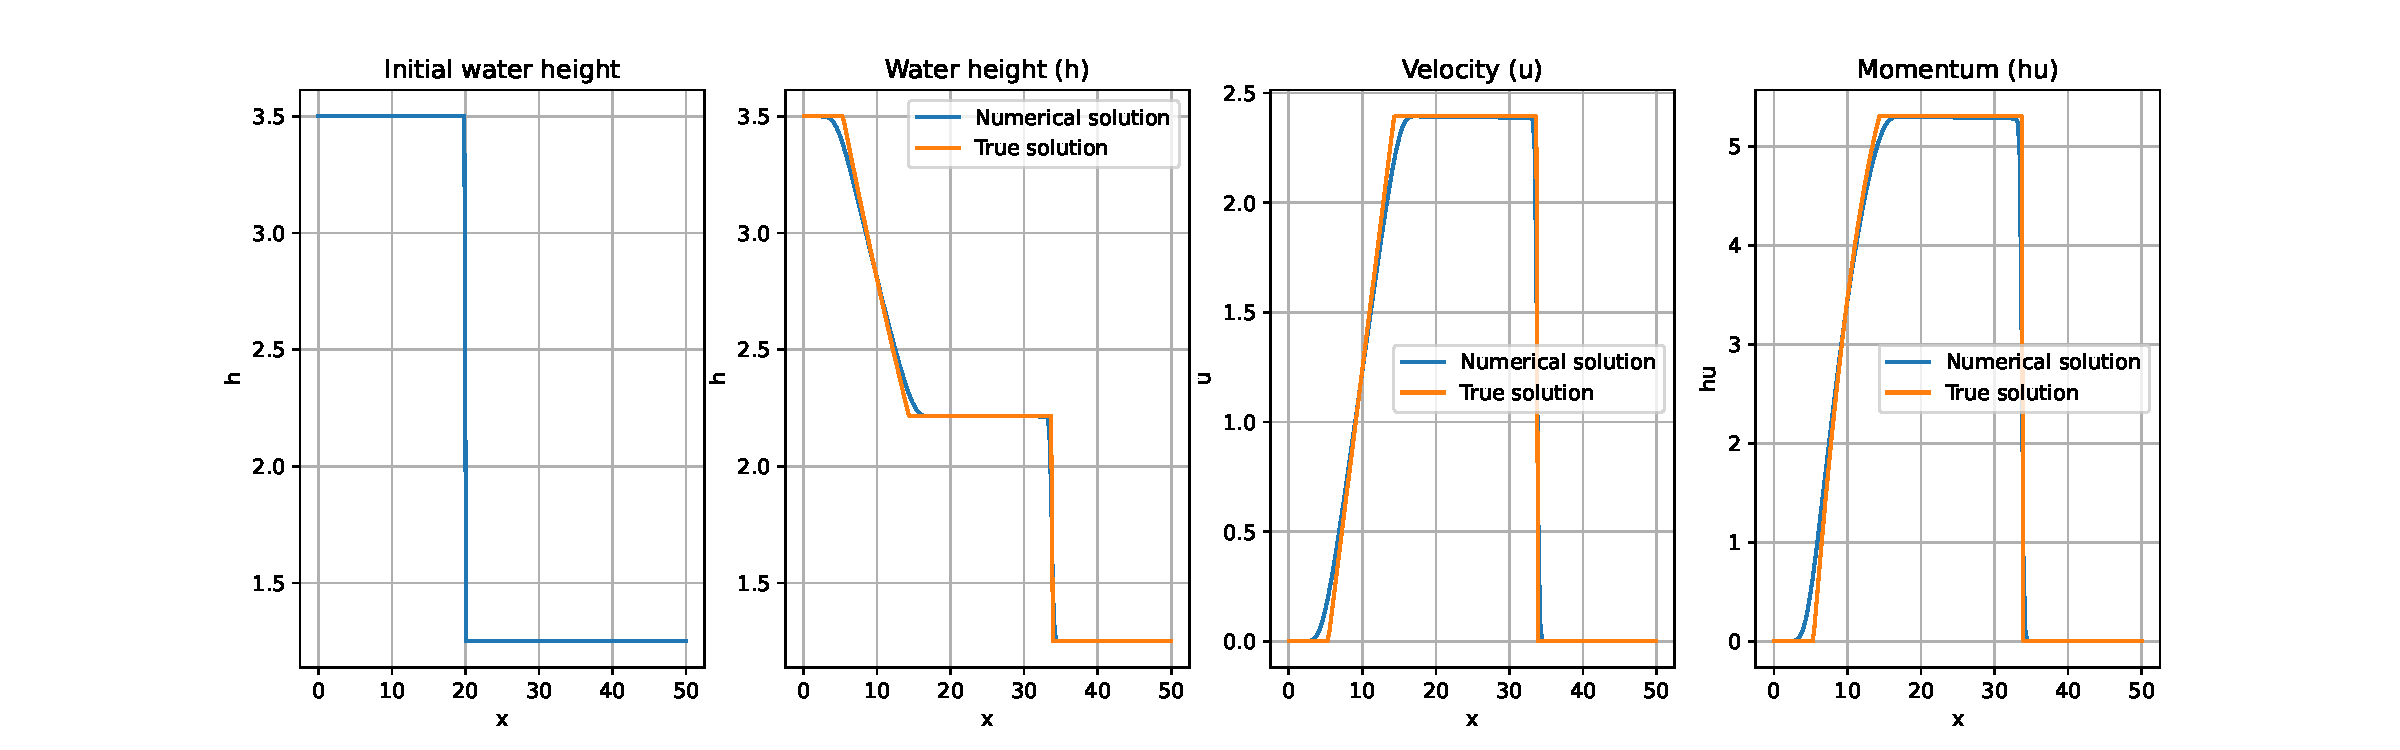
\includegraphics[width=0.99\textwidth]{C:/Users/Matteo/Shallow-Water-Equations/plots/sol_1D_val.pdf}
    \caption{The initial water height $h$ at $t=0$ s, together with the water height $h$, the fluid velocity $u$ and the momentum $hu$ at $t=2.5$ s.}\label{fig:1D_dam_break}
\end{figure}
From \autoref{fig:1D_dam_break} we see that the numerical solution aligns well with the true solution, and overall successfully captures the discontinuity.
We also see that the solution consists of a right shock wave and a left rarefaction wave, as expected from the initial conditions.
This is seen as, the shock wave to the right has a high speed and represent a discontinuity in the solution for the water height.
The rarefaction wave to the left is a smooth transition from the high water height to a lower water height.

\section{Toro test cases}\label{sec:toro_test_cases}
We have tested the FVM on the five test cases for Riemann problems from Toro (2001)~\cite{Toro2001-Shock}.
The initial conditions for the five test cases are given in \autoref{tab:toro_test_cases}.
\begin{table}[H]
    \centering
    \begin{tabular}{c|c|c|c|c|c|c}
        \hline
        \textbf{Test case} & \textbf{$h_L$} [m] & \textbf{$u_L$} [m/s] & \textbf{$h_R$} [m] & \textbf{$u_R$} [m/s] & \textbf{$x_0$} [m] & \textbf{$t_{end}$} [s] \\
        \hline\hline
        1 & 1.0 & 2.5 & 0.1 & 0.0 & 10.0 & 7.0 \\
        2 & 1.0 & -5.0 & 1.0 & 5.0 & 25.0 & 2.5 \\
        3 & 1.0 & 0.0 & 0.0 & 0.0 & 20.0 & 4.0 \\
        4 & 0.0 & 0.0 & 1.0 & 0.0 & 30.0 & 4.0 \\
        5 & 0.1 & -3.0 & 0.1 & 3.0 & 25.0 & 5.0 \\
        \hline
    \end{tabular}
    \caption{Initial conditions for the five test cases.}\label{tab:toro_test_cases}
\end{table}
The domain is $x \in [0 \text{ m}, 50 \text{ m}]$ for all test cases.
The Riemann problems are chosen to test the numerical method on different combinations of shock waves and rarefaction waves.
We solved the test cases using the following fluxes: 
\begin{enumerate}
    \item Godunov method with exact Riemann solver,
    \item Lax-Friedrich flux,
    \item Lax-Wendroff flux,
    \item FORCE flux,
    \item HLL flux.
\end{enumerate}

\subsection*{Test case 1}
The initial conditions for test case 1 are visualised in \autoref{fig:toro_test1_initial} and the solution after $t=7.0$ s is given in \autoref{fig:toro_test1_final}.
\begin{figure}[H]
    \centering
    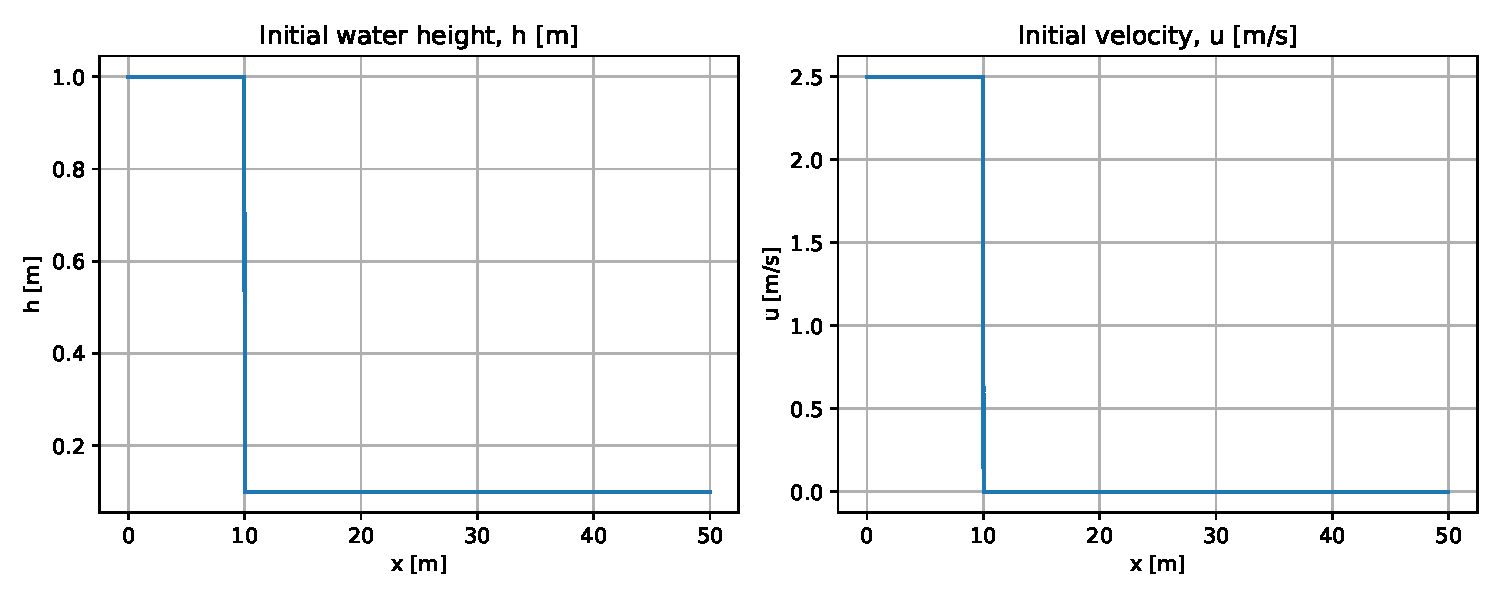
\includegraphics[width=0.8\textwidth]{C:/Users/Matteo/Shallow-Water-Equations/plots/toro_test1_initial.pdf}
    \caption{Initial conditions for the test case.}\label{fig:toro_test1_initial}
\end{figure}
\begin{figure}[H]
    \centering
    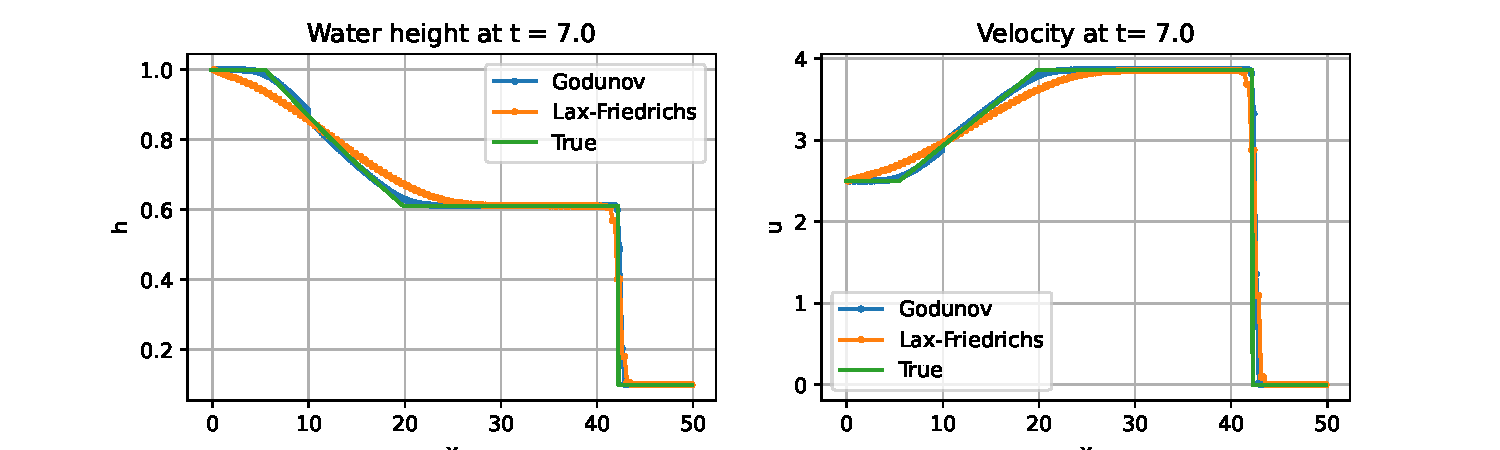
\includegraphics[width=0.65\textwidth]{C:/Users/Matteo/Shallow-Water-Equations/plots/toro_test1_final.pdf}
    \caption{Final solution for the test case after $t=7.0$ s.}\label{fig:toro_test1_final}
\end{figure}
For this test case all the fluxes work well, but there are minor differences in the solution, which can be seen in \autoref{fig:toro_test1_final}.
For instance, we see that the Lax-Wendroff (LW) flux has some oscillations in the solution at the discontinuity, which is not present in the other fluxes.
Individual plots for the different fluxes can be found in \autoref{fig:toro_test1_fluxes} in Appendix~\ref{app:toro_test_case_1}.
Similarly to the case of the 1D dam break problem in \autoref{sec:1D_dam_break}, we see that the solution consists of a right shock wave and a left rarefaction wave.

\newpage
\subsection*{Test case 2}
The initial conditions for test case 2 are illustrated in \autoref{fig:toro_test2_initial}.
\begin{figure}[H]
    \centering
    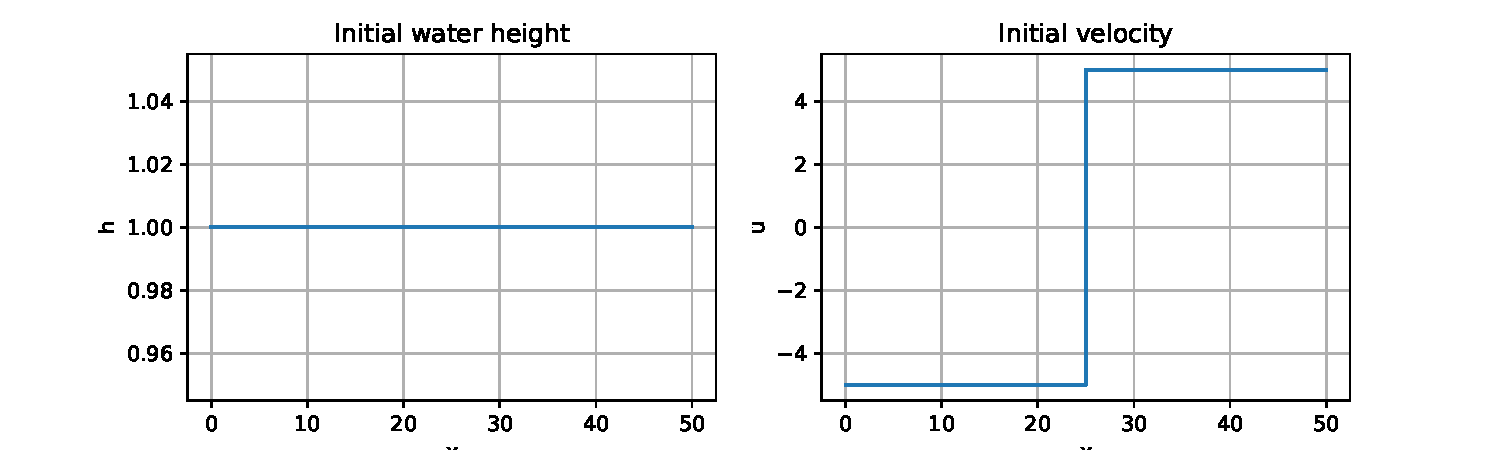
\includegraphics[width=0.8\textwidth]{C:/Users/Matteo/Shallow-Water-Equations/plots/toro_test2_initial.pdf}
    \caption{Initial conditions for the test case.}\label{fig:toro_test2_initial}
\end{figure}
The solution after $t = 2.5$ s is illustrated in \autoref{fig:toro_test2_final}.
\begin{figure}[H]
    \centering
    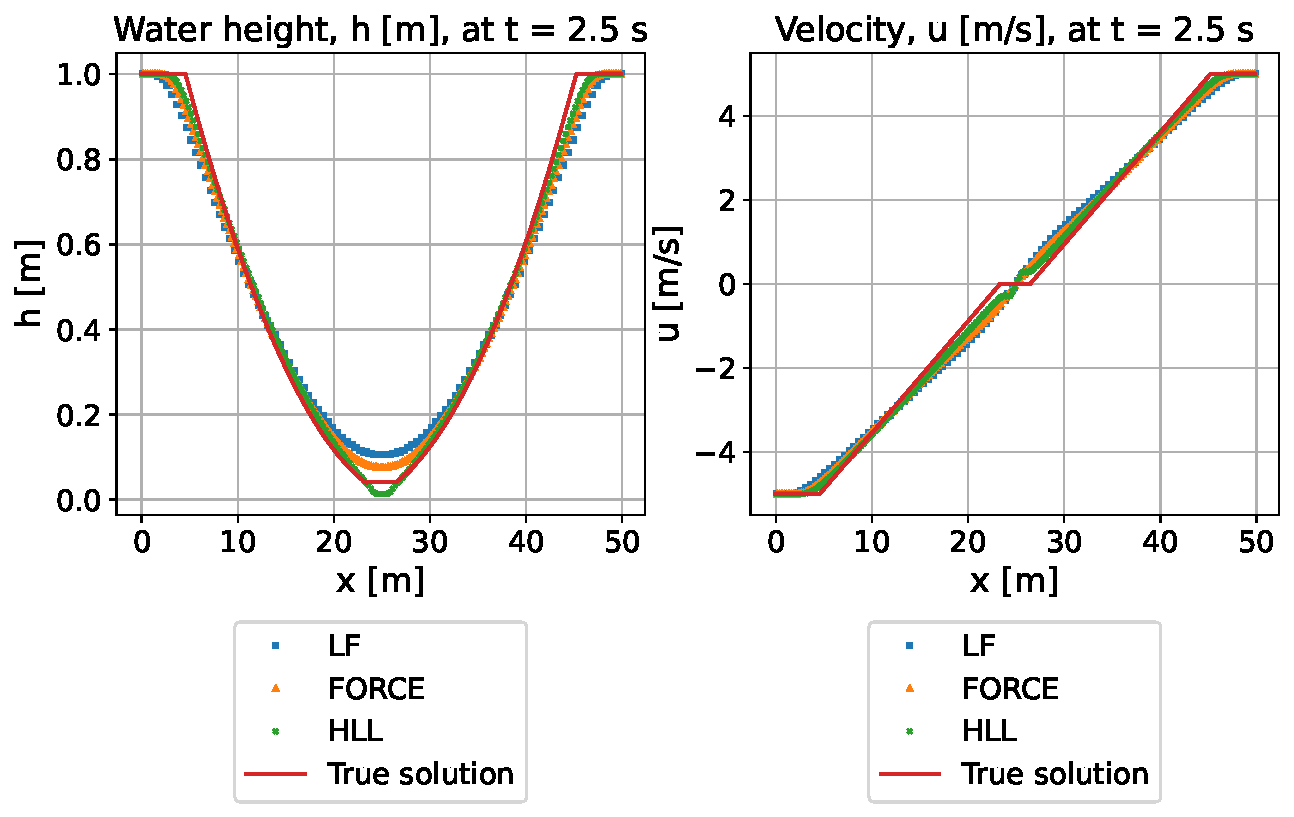
\includegraphics[width=0.65\textwidth]{C:/Users/Matteo/Shallow-Water-Equations/plots/toro_test2_final.pdf}
    \caption{Final solution for the test case after $t = 2.5$ s.}\label{fig:toro_test2_final}
\end{figure}
In test case 2 we have two rarefaction waves, one on the left side and one on the right side of $x_0$.
As they are travelling in opposite directions (away from each other), due to the initial velocity, there will be created a nearly dry bed in the middle of the domain.
Many methods have difficulties with this test case as they may compute a negative water height.
For these experiments we were able to get close to the true solution, using Lax-Friedrich flux, FORCE flux and HLL flux.
The results for the different fluxes can be found in \autoref{fig:toro_test2_fluxes} in Appendix~\ref{app:toro_test_case_2}.
For the fluxes, Godunov method with exact Riemann solver, and Lax-Wendroff, it was not possible to get an acceptable solution.
Among the LF, FORCE and HLL fluxes we also see differences in how close the numerical solution comes to $h = 0$ m at $x = 25$ m.

\newpage
\subsection*{Test case 3}
The initial conditions for test case 3 are given in \autoref{fig:toro_test3_initial}.
\begin{figure}[H]
    \centering
    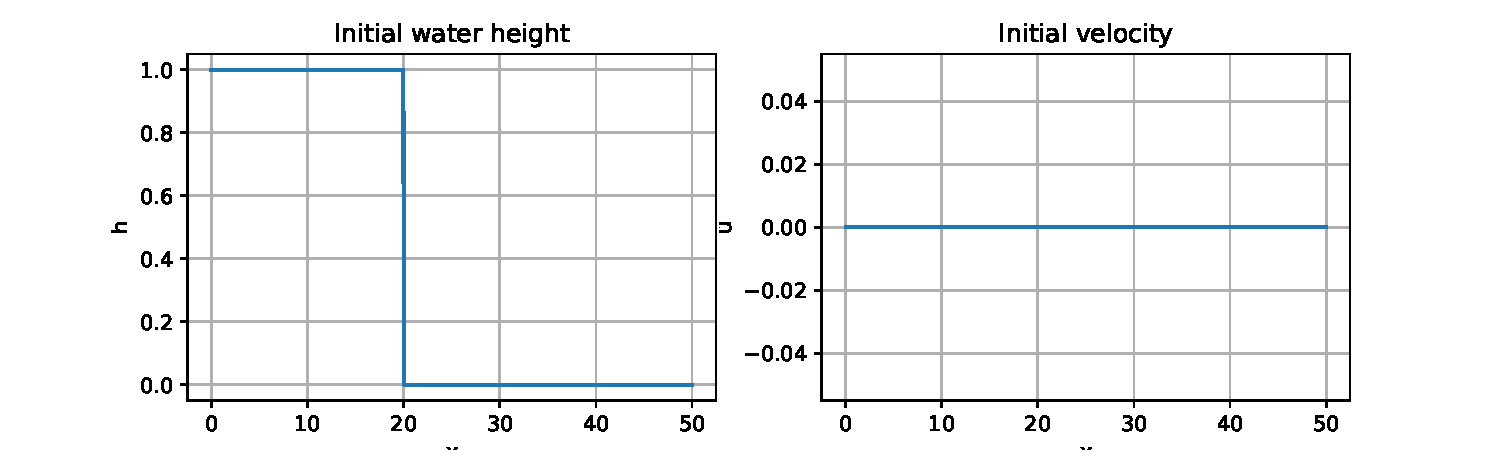
\includegraphics[width=0.8\textwidth]{C:/Users/Matteo/Shallow-Water-Equations/plots/toro_test3_initial.pdf}
    \caption{Initial conditions for the test case.}\label{fig:toro_test3_initial}
\end{figure}
In \autoref{fig:toro_test3_initial} we see that this is a dam break problem, as the initial velocity is zero everywhere.
The solution after $t=4.0$ s is given in \autoref{fig:toro_test3_final}.
\begin{figure}[H]
    \centering
    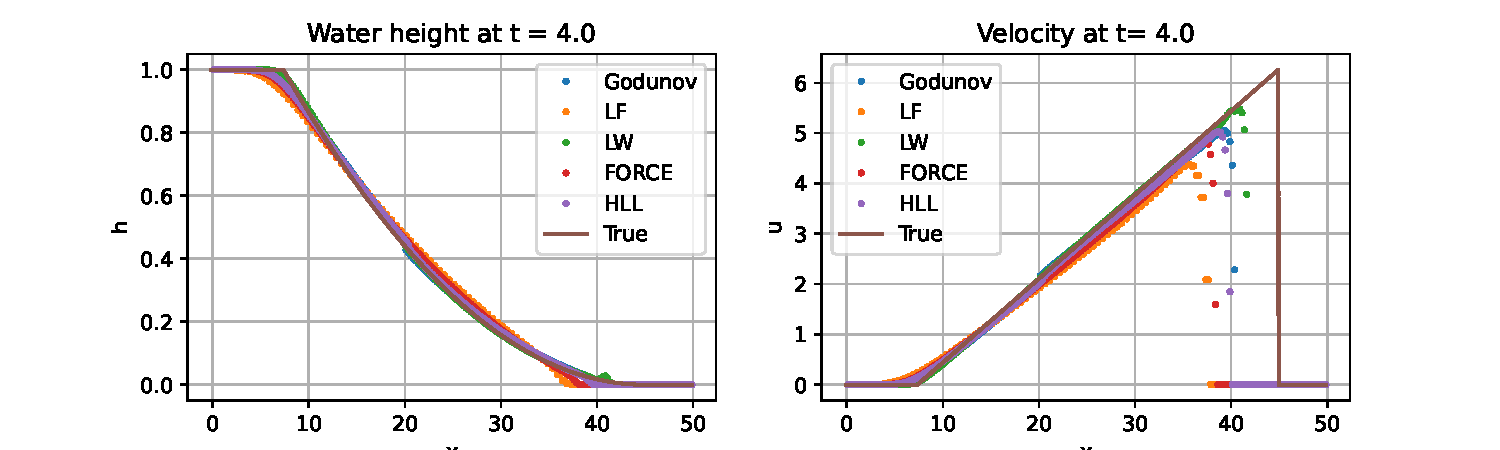
\includegraphics[width=0.65\textwidth]{C:/Users/Matteo/Shallow-Water-Equations/plots/toro_test3_final.pdf}
    \caption{Final solution for the test case after $t = 4.0$ s.}\label{fig:toro_test3_final}
\end{figure}
In case 3, we face a dry-bed region on the right side of the domain.
To handle this with the FVM, a small value is added to $h_R$, as the method struugles with $h_R = 0$ m.
We set $h_R = 0.00005$ m for numerical stability, but the true solution is for $h_R = 0$ m.
Experiments show the solution converges to the true solution as $h_R$ approaches 0.
As shown in \autoref{fig:toro_test3_final}, there are differences in velocity prediction performance across the fluxes.
All fluxes are visualised in \autoref{fig:toro_test3_fluxes} in Appendix~\ref{app:toro_test_case_3}, with the Lax-Wendroff (LW) flux providing the closest velocity solution.

\newpage
\subsection*{Test case 4}
The initial conditions for test case 4 are given in \autoref{fig:toro_test4_initial}, and the solution after $t=4.0$ s is given in \autoref{fig:toro_test4_final}.
\begin{figure}[H]
    \centering
    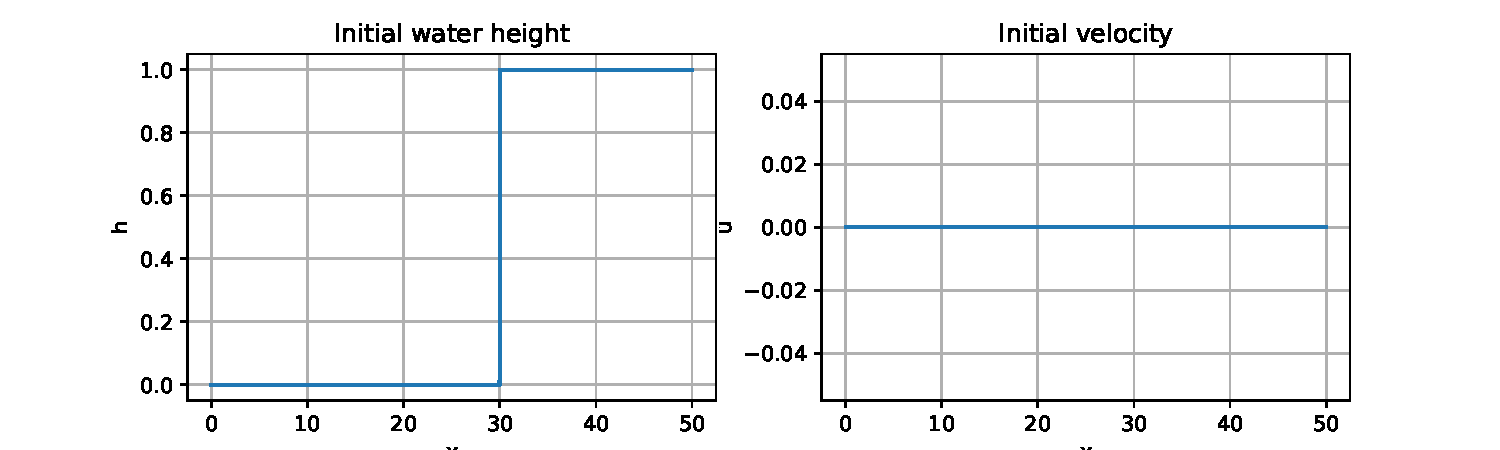
\includegraphics[width=0.8\textwidth]{C:/Users/Matteo/Shallow-Water-Equations/plots/toro_test4_initial.pdf}
    \caption{Initial conditions for the test case.}\label{fig:toro_test4_initial}
\end{figure}

\begin{figure}[H]
    \centering
    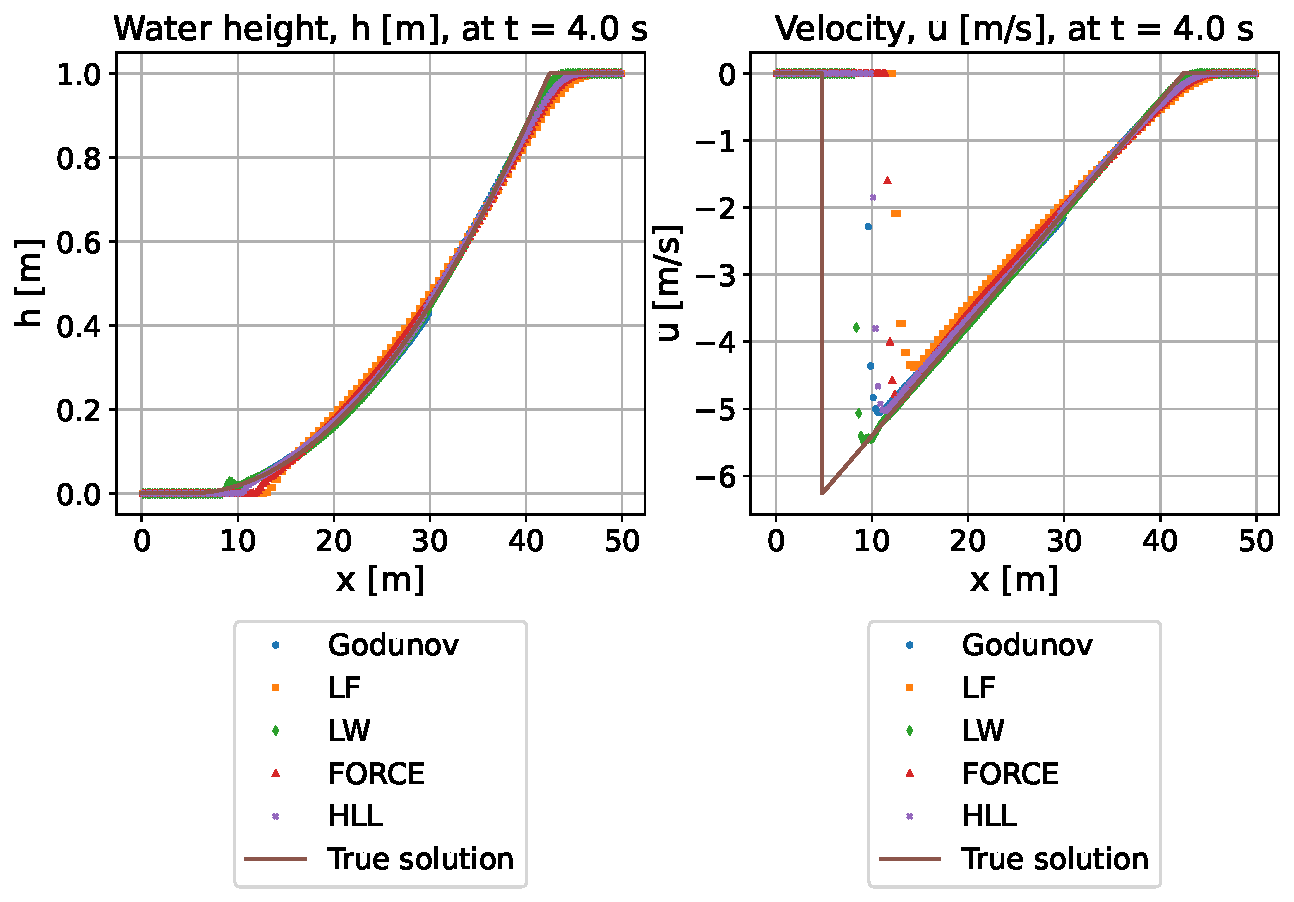
\includegraphics[width=0.65\textwidth]{C:/Users/Matteo/Shallow-Water-Equations/plots/toro_test4_final.pdf}
    \caption{Final solution for the test case after $t = 4.0$ s.}\label{fig:toro_test4_final}
\end{figure}
This test problem is symmetric to test case 3, meaning we face the same challenges of a dry-bed region, now located in the left part of the domain.
We set $h_L = 0.00005$ m, and the solution converges to the true solution as $h_L$ approaches 0.
This case is included to test if the results are as expected.
As in test case 4, we observe differences in the fluxes performance, and again we observe that the Lax-Wendroff (LW) flux comes closest to the true solution for the velocity.
The results for the different fluxes can be found in \autoref{fig:toro_test4_fluxes} in Appendix~\ref{app:toro_test_case_4}.

\newpage
\subsection*{Test case 5}
The initial conditions for test case 5 are given in \autoref{fig:toro_test5_initial}, and the final solution after $t=5.0$ s is given in \autoref{fig:toro_test5_final}.
\begin{figure}[H]
    \centering
    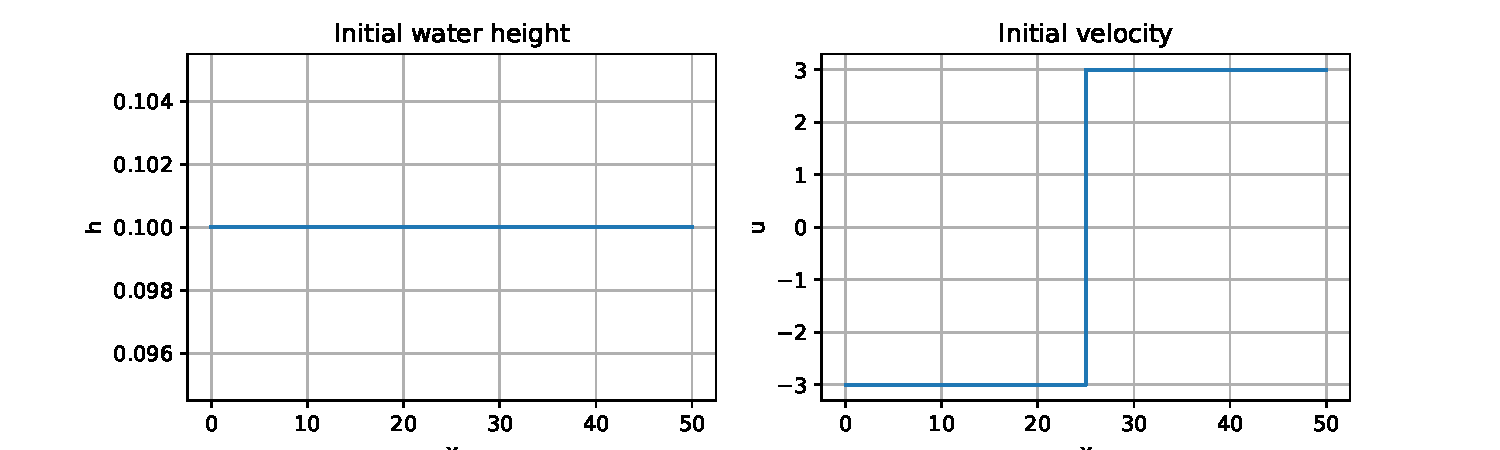
\includegraphics[width=0.8\textwidth]{C:/Users/Matteo/Shallow-Water-Equations/plots/toro_test5_initial.pdf}
    \caption{Initial conditions for the test case.}\label{fig:toro_test5_initial}
\end{figure}

\begin{figure}[H]
    \centering
    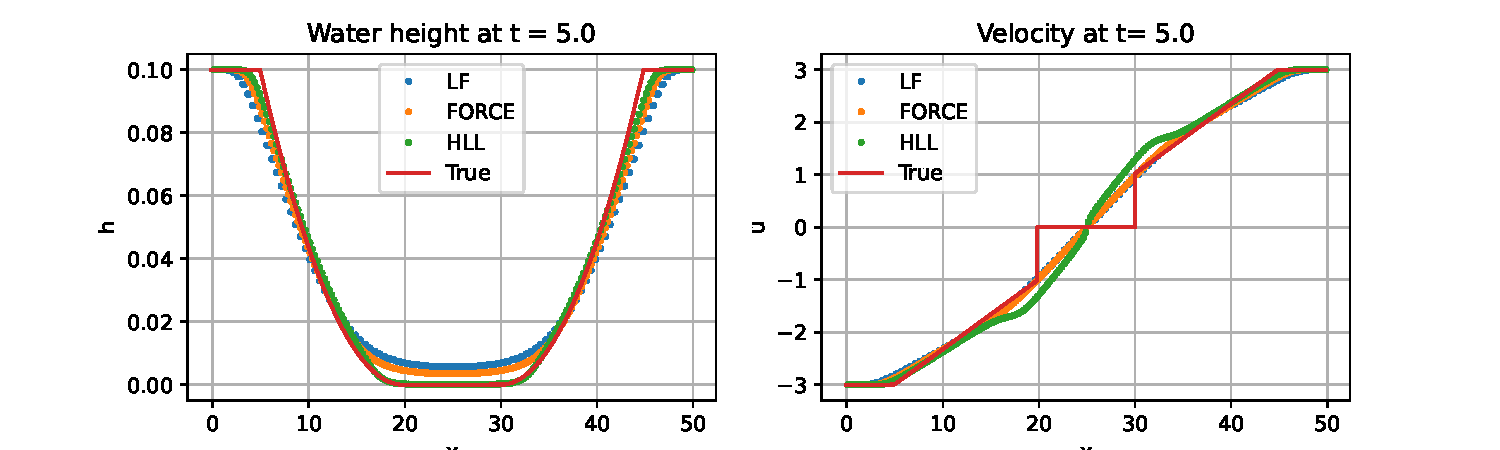
\includegraphics[width=0.65\textwidth]{C:/Users/Matteo/Shallow-Water-Equations/plots/toro_test5_final.pdf}
    \caption{Final solution for the test case after $t = 5.0$ s.}\label{fig:toro_test5_final}
\end{figure}
From~\autoref{fig:toro_test5_final} we see that the numerical solution for the velocity $v$ at $t=5.0$ s is smooth, where the true solution is discontinuous. 
In this test case there are also challenges with some of the fluxes due to the generation of a dry-bed region in the middle of the domain.
The fluxes that are not able to solve this case are: the Godunov method with exact Riemann solver and the Lax-Wendroff flux, the same as in test case 2.
Individual plots for the different fluxes can be found in \autoref{fig:toro_test5_fluxes} in Appendix~\ref{app:toro_test_case_5}, where we see that the HLL flux provides the best solution for the water height.
The solution consists of two rarefaction waves, one on the left side and one on the right side, and a dry-bed region in the middle.
To get an overview of which fluxes that were able to produce solutions for the test cases, consider~\autoref{tab:toro_fluxes}.
\begin{table}[H]
    \centering
    \begin{tabular}{c|c|c|c|c|c}
        \hline
        \textbf{Test case} & \textbf{Godunov} & \textbf{LF} & \textbf{LW} & \textbf{FORCE} & \textbf{HLL}   \\
        \hline\hline
        1 & $\checkmark$ & $\checkmark$ & $\checkmark$ & $\checkmark$ & $\checkmark$   \\
        2 & $\times$ & $\checkmark$ & $\times$ & $\checkmark$ & $\checkmark$ \\
        3 & $\checkmark$ & $\checkmark$ & $\checkmark$ & $\checkmark$ & $\checkmark$  \\
        4 & $\checkmark$ & $\checkmark$ & $\checkmark$ & $\checkmark$ & $\checkmark$  \\
        5 & $\times$ & $\checkmark$ & $\times$ & $\checkmark$ & $\checkmark$  \\
        \hline
    \end{tabular}
    \caption{Overview of which fluxes that were able to produce solutions for the test cases.}\label{tab:toro_fluxes}
\end{table}
Note, that as we see in the results, there are still differences in the solutions accuracy between the fluxes that were able to solve the test cases.
 
\section{The 1D linearized Shallow Water Equations on a sphere}\label{sec:1D_sphere}
In this section we consider the 1D LSWE on a sphere.
We consider the spatial dimension $\theta$, which is the longitude angle and keep the latitude $\phi$ constant.
The LSWE on a sphere are given by~\eqref{eq:linearized_swe_spherical} with the initial conditions given by~\eqref{eq:1D_swe_spherical_ic}.
The LSWE on a sphere are solved using the FVM with the ERK4 time-stepping method.
The initial conditions, together with the solution after $t = 0.25$ s and $t = 0.31$ s are visualised in \autoref{fig:1D_LSWE_sphere}.
\begin{figure}[H]
    \centering
    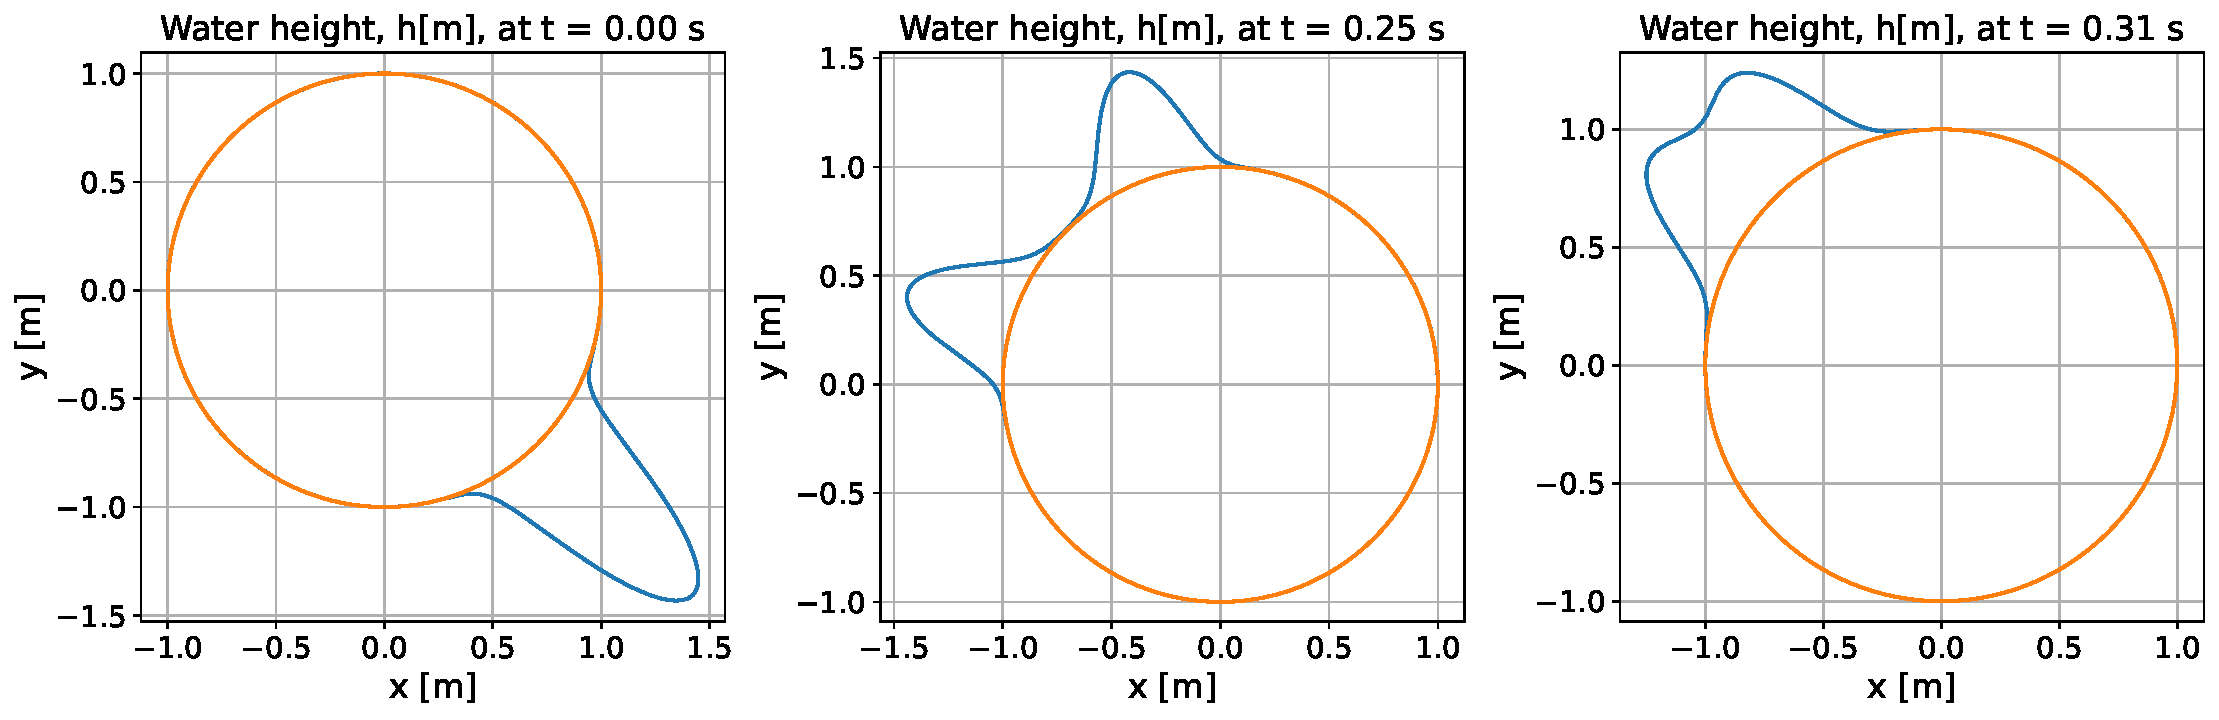
\includegraphics[width=0.9\textwidth]{C:/Users/Matteo/Shallow-Water-Equations/plots/1D_LSWE_sphere_time_steps.pdf}
    \caption{The water height, $h[m]$, at $t = 0$ s, $t = 0.25$ s and $t = 0.31$ s.}\label{fig:1D_LSWE_sphere}
\end{figure}
From \autoref{fig:1D_LSWE_sphere} we see how the water height evolves over time.
We observe that the initial wave split into two waves, travelling in opposite directions.
When the two waves meet, we see how the periodic boundary conditions operate, as the waves are melting together, and then split again into two waves, as in the beginning.
This is more clear visualised in the animation for this case, a link and qr-code can be found in \autoref{fig:2D_dam_break_qr_all}.
Since we do not account for friction and have neglecting external forces except gravity, the waves will continue to travel around the sphere.
In this case we do not have a true solution to compare with, but the numerical solution seems reasonable.

\section{The 2D idealised Circular Dam Break Problem}\label{sec:2D_dam_break}
We now proceed to the 2D case, considering an idealised circular dam break problem over a horizontal bottom, a problem from Toro (2024)~\cite{Toro2024}.
We assume there is an infinitely thin circular wall at radius $R = 2.5$ m in a square domain of size $40 \text{ m} \times 40 \text{ m}$ with centre at $(x_c,y_c) = (20 \text{ m}, 20 \text{ m})$.
The initial velocity is zero, and the initial water height is $2.5$ m inside the circle and $0.5$ m outside the circle, as given by the following initial conditions:
\begin{align*}
    h(x,y,0) &= \begin{cases}
        2.5 \text{ m}, & \text{if } \sqrt{ {(x-x_c)}^2 + {(y-y_c)}^2 } \leq R, \\
        0.5 \text{ m}, & \text{otherwise},
    \end{cases} \\
    u(x,y,0) &= 0 \text{ m/s}, \\
    v(x,y,0) &= 0 \text{ m/s}.
\end{align*}
We use a mesh of size $64 \times 64$.
The boundary conditions simulate a wall, enforcing zero flux at the boundary and causing the flow to bounce back into the domain.
The problem is solved using the FVM with the Rusanov flux, and the results after $t=0.0 \text{ s}, 0.4 \text{ s}, 0.7 \text{ s}$ and $1.4$ s are visualised in \autoref{fig:2D_dam_break_grid}.
\begin{figure}[H]
    \centering
    \begin{subfigure}{0.49\textwidth}
        \centering
        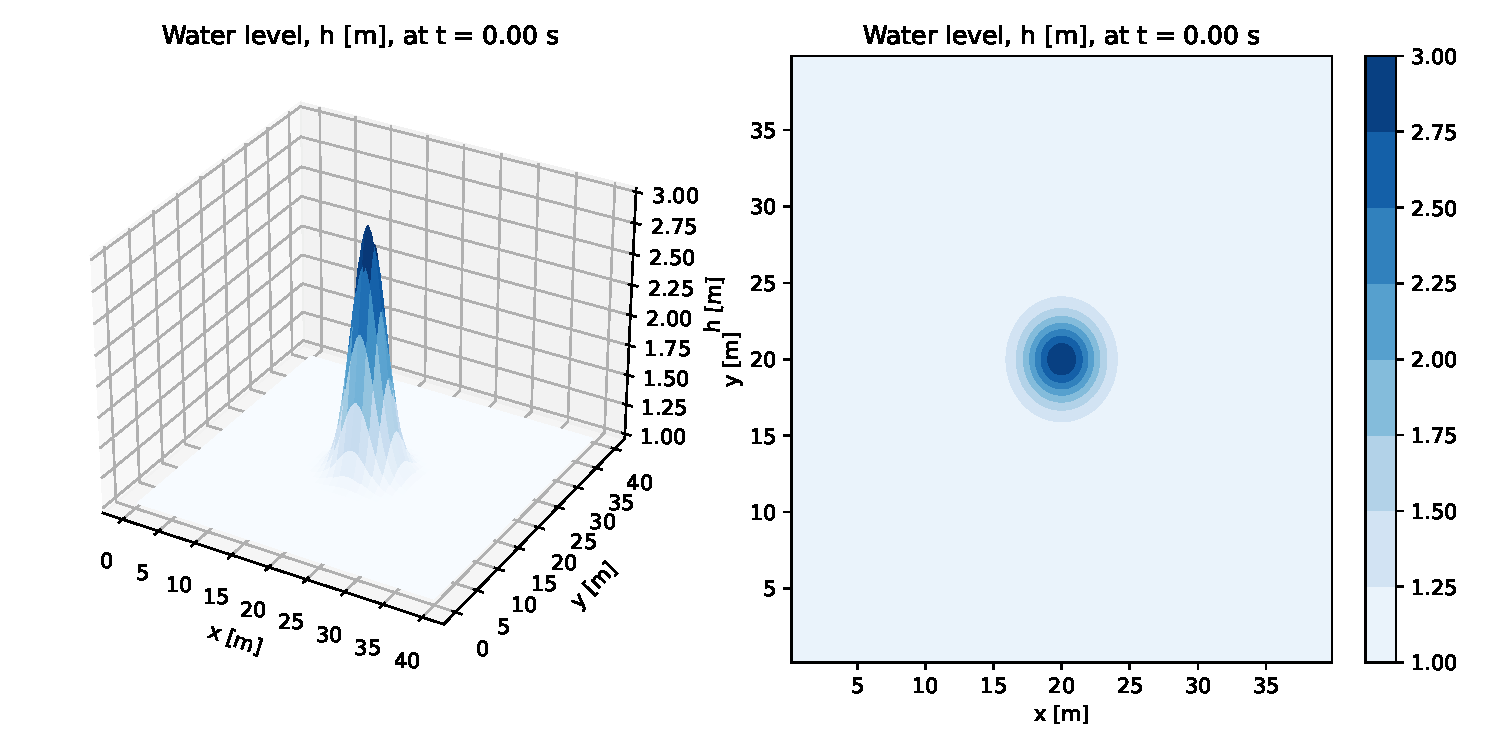
\includegraphics[width=\textwidth]{C:/Users/Matteo/Shallow-Water-Equations/plots/toro2D_t=0.pdf}
        \caption{2D dam break problem after $t=0$ s.}\label{fig:2D_dam_break_t0}
    \end{subfigure}
    \hfill
    \begin{subfigure}{0.49\textwidth}
        \centering
        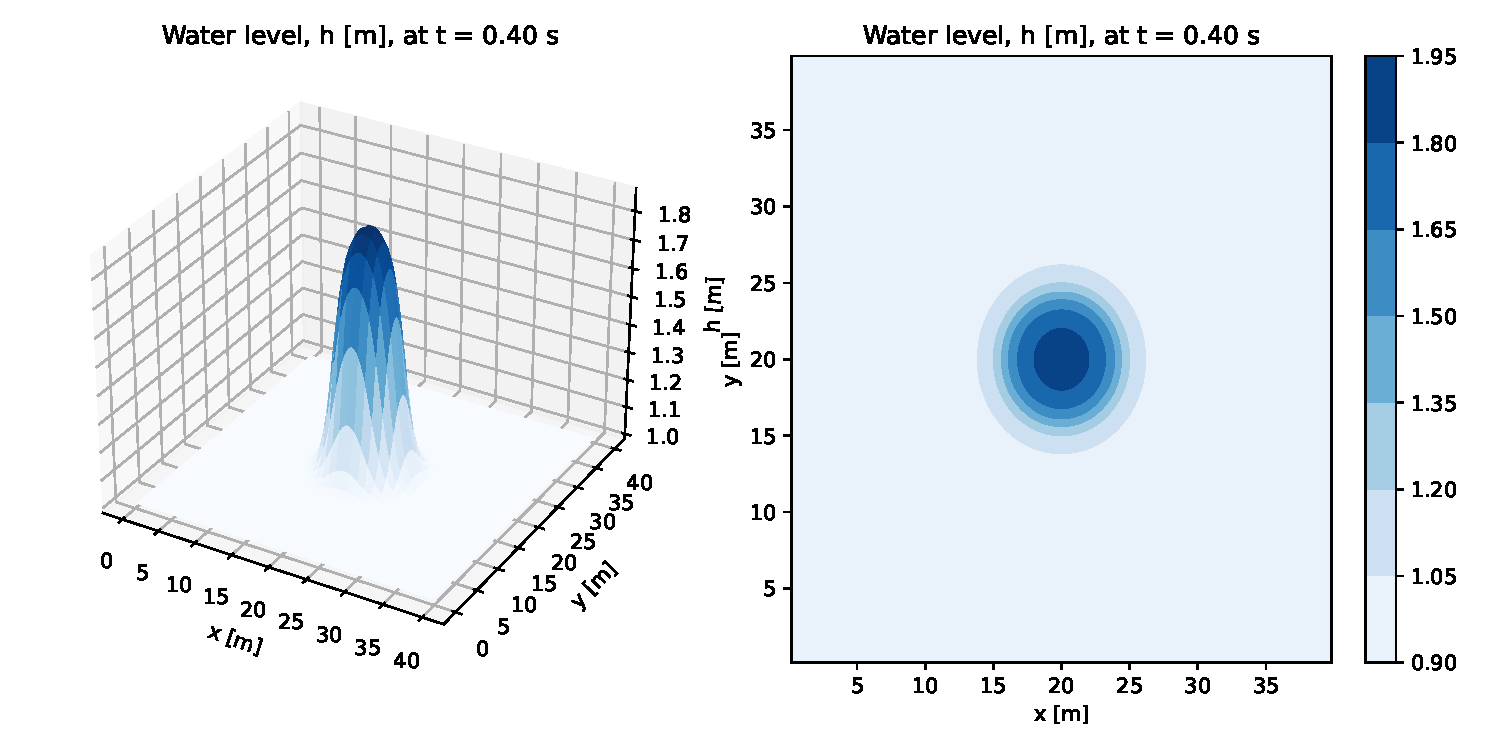
\includegraphics[width=\textwidth]{C:/Users/Matteo/Shallow-Water-Equations/plots/toro2D_t=0.4.pdf}
        \caption{2D dam break problem after $t=0.4$ s.}\label{fig:2D_dam_break_t0.4}
    \end{subfigure}

    \vspace{0.5cm} % Adjusts vertical space between rows

    \begin{subfigure}{0.49\textwidth}
        \centering
        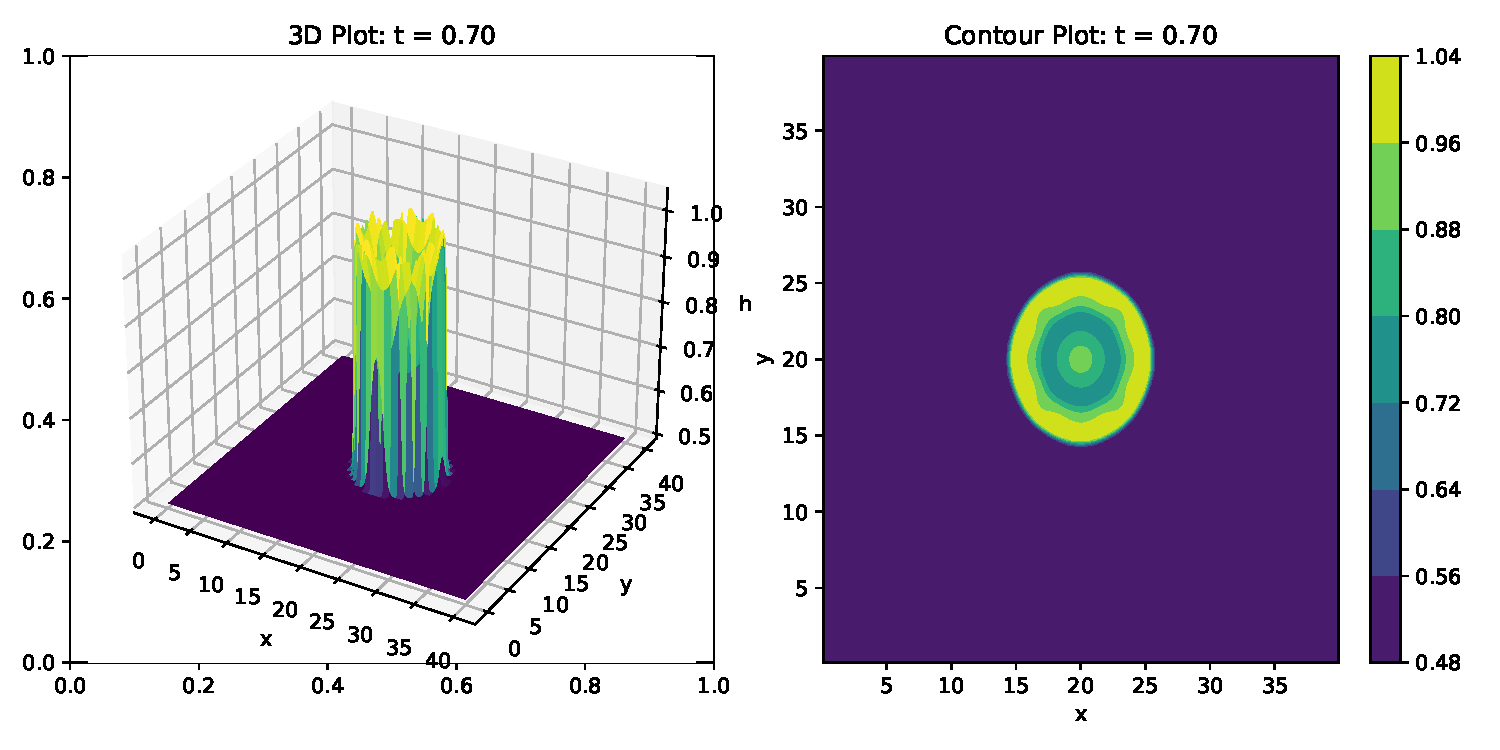
\includegraphics[width=\textwidth]{C:/Users/Matteo/Shallow-Water-Equations/plots/toro2D_t=0.7.pdf}
        \caption{2D dam break problem after $t=0.7$ s.}\label{fig:2D_dam_break_t0.7}
    \end{subfigure}
    \hfill
    \begin{subfigure}{0.49\textwidth}
        \centering
        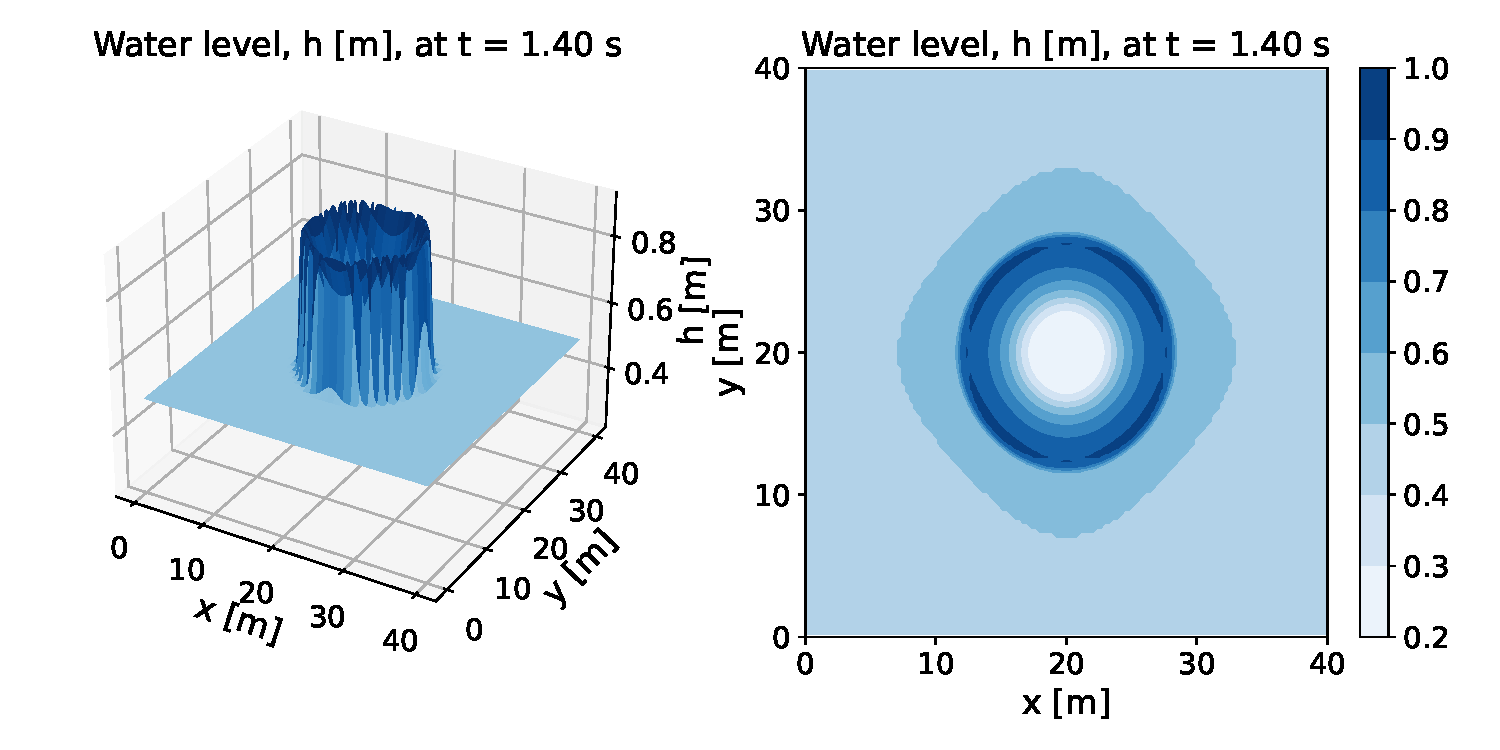
\includegraphics[width=\textwidth]{C:/Users/Matteo/Shallow-Water-Equations/plots/toro2D_t=1.4.pdf}
        \caption{2D dam break problem after $t=1.4$ s.}\label{fig:2D_dam_break_t1.4}
    \end{subfigure}

    \caption{Snapshots of the 2D dam break problem at different times.}\label{fig:2D_dam_break_grid}
\end{figure}
By comparing \autoref{fig:2D_dam_break_grid} with the results from Toro (2024)~\cite{Toro2024}, we see that the numerical solution aligns well with the true solution.


\section{Scalability}\label{sec:scalability}
Numerical methods are good as they can be more or less as accurate as we want them to be, but the computational cost increases with the number of cells, i.e., the more high-resolution grid we use.
Previoulsy in the thesis, we have indicated that a disadvantage of the FVM is that the computational cost increases with the number of cells.
To test the scalability of the FVM to solve the 2D SWE, we have solved the 2D SWE with a Gaussian initial condition, as described in \autoref{ch:method}, for different values of $N$, i.e., the number of cells in each direction, and measured the run time.
The results are presented in \autoref{tab:scalability}.
\begin{table}[H]
    \centering
    \begin{tabular}{c|ccccc}
        \hline
        $N$ & 16 & 32 & 64 & 128 & 256 \\
        \hline 
        Time [$s$] & 
        \input{C:/Users/Matteo/Shallow-Water-Equations/saved_results/2D_FVM_N=16_time_5.txt} &
        \input{C:/Users/Matteo/Shallow-Water-Equations/saved_results/2D_FVM_N=32_time_5.txt} &
        \input{C:/Users/Matteo/Shallow-Water-Equations/saved_results/2D_FVM_N=64_time_5.txt} &
        \input{C:/Users/Matteo/Shallow-Water-Equations/saved_results/2D_FVM_N=128_time_5.txt} &
        \input{C:/Users/Matteo/Shallow-Water-Equations/saved_results/2D_FVM_N=256_time_5.txt}
        \\
        \hline
    \end{tabular}
    \caption{Running time for the FVM to solve 2D SWE for different values of $N$.}\label{tab:scalability}
\end{table}
The run time $[s]$ dependent on the number of cells $N$ is illustrated in \autoref{fig:scalability_FVM_2D}.
\begin{figure}[H]
    \centering
    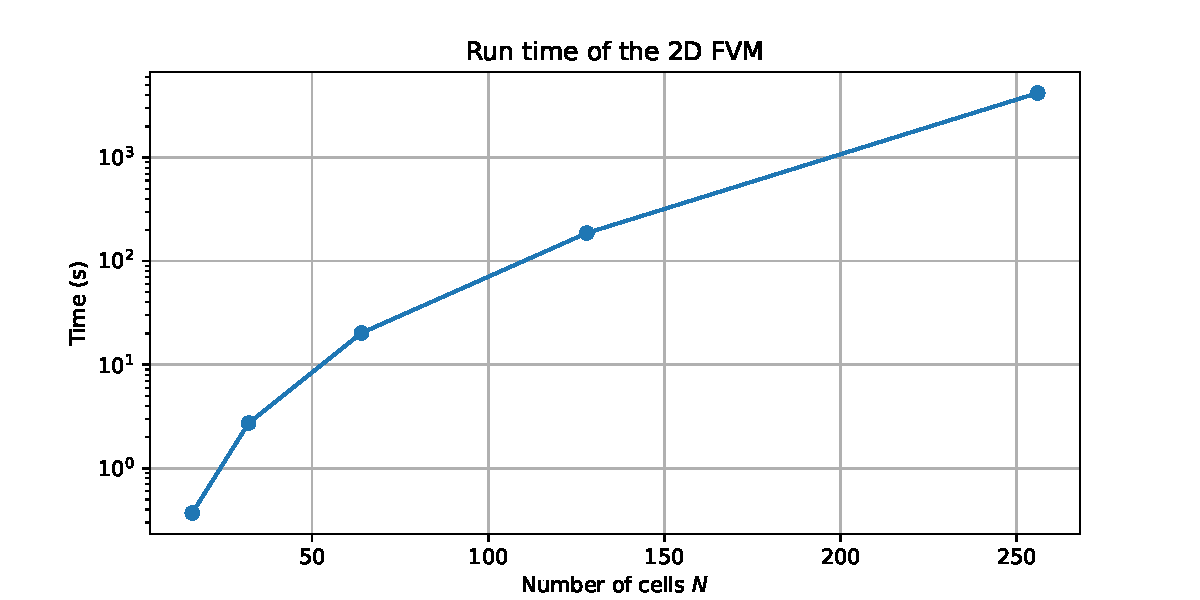
\includegraphics[width=0.8\textwidth]{C:/Users/Matteo/Shallow-Water-Equations/plots/scalability_FVM_2D.pdf}
    \caption{Run time $[s]$ of the 2D FVM to solve the SWE, depending on number of grid cells $N$.
            Note that the axis with time is in log-scale.}\label{fig:scalability_FVM_2D}
\end{figure}
From \autoref{tab:scalability} and \autoref{fig:scalability_FVM_2D} we see that the run time increases drastically as the number of cells, $N$, grows.
This behavior is expected since an increase in the number of cells leads to a higher number of computations.
Additionally, the computational cost is further amplified by an increase in the number of time steps.
This occurcs because the time step size decreases as the number of cells increases, due to the CFL condition, as seen in~\eqref{eq:CFL_number}.

As a result, the computational time escalates rapidly, reducing the scalability of the FVM for real-world simulations.
To effectively model phenomena such as floods or tsunamis, we need a scalable method.
This challenge motivates the exploration of data-driven methods, as we aim to investigate whether they offer a more scalable solution.

\section{Animations}\label{sec:animations}
To visualise the results of the numerical experiments, we have created some animations.
These include an animation of the 1D LSWE on a sphere, demonstrating the periodic boundary conditions.
There are also animations for the 2D idealised circular dam break problem and the 2D SWE with a Gaussian initial condition projected on a sphere, as described in \autoref{sec:data_generation_sphere}.
The following QR-codes provide access to the animations.
A link to the animations is also provided in the caption of \autoref{fig:2D_dam_break_qr_all}, directing to a dedicated GitHub repository.
\begin{figure}[H]
    \centering
    \begin{subfigure}{0.25\textwidth}
        \begin{minipage}[t]{\textwidth}
            \centering
            
\includegraphics[width=\textwidth]{C:/Users/Matteo/Shallow-Water-Equations/QR/1D_LSWE_sphere_17012025.gif_qr.png}
            \caption{QR-code for the 1D LSWE on a sphere.}\label{fig:1D_LSWE_sphere_qr}
        \end{minipage}
    \end{subfigure}
    \hspace{1cm}
    \begin{subfigure}{0.25\textwidth}
        \begin{minipage}[t]{\textwidth}
            \centering
            
\includegraphics[width=\textwidth]{C:/Users/Matteo/Shallow-Water-Equations/QR/toro2D_dambreak_FVM_17012025_N=64_t=10_qr.png}
            \caption{QR-code for the 2D idealized circular dam break problem.}\label{fig:2D_dam_break_qr}
        \end{minipage}
    \end{subfigure}
    \hspace{1cm}
    \begin{subfigure}{0.25\textwidth}
        \begin{minipage}[t]{\textwidth}
            \centering
            
\includegraphics[width=\textwidth]{C:/Users/Matteo/Shallow-Water-Equations/QR/sphere_gaussian_FVM_17012025_qr.png}
            \caption{QR-code for the 2D SWE with initial Gaussian conditions, projected on a sphere.}\label{fig:2D_dam_break_qr_part2}
        \end{minipage}
    \end{subfigure}
    \caption{QR-codes for the animations.
            All animations can be found at: \url{https://github.com/MelissaJessen/Shallow-Water-Equations-Animations/blob/main/README.md}.}\label{fig:2D_dam_break_qr_all}
\end{figure}
In the animation for the 2D idealised circular dam break problem, we observe what happens after the time steps in \autoref{fig:2D_dam_break_grid}.
We note that when the waves hit the boundaries, they are reflected back into the domain, demonstrating the behaviour of the boundary conditions.
In the animation for the 2D SWE with a Gaussian initial condition on a sphere, we note that since the SWE are solved in a 2D cartesian domain and wrapped to a sphere, we observe non-physical behaviour, especially close to the poles.
